\section{Einleitung}
%Security and Privacy in Cloud Computing: Aktuelle Herausforderungen

%Es wird immer wieder fehlende Sicherheit und fehlender Schutz privater Daten in der %Cloud als Hauptargument genannt, warum Firmen die öffentliche Cloud nicht nutzen %wollen. Was wären die aktuelle Herausforderungen und eventeulle Lösungsansätze?

Cloud Computing erlaubt es bei Bedarf über ein Netz auf einen geteilten Pool von konfigurierbaren Ressourcen wie weiteren Netzen, Speicher, Anwendungen, Servern und Diensten zuzugreifen. Diese Ressourcen können dabei schnell und mit minimalem Verwaltungsaufwand zur Verfügung gestellt werden \cite{mell2011}. 
Durch diese Eigenschaften des Cloud Computing ergeben sich die folgenden Vorteile \cite{ganesh2014}:
\begin{itemize}
\item 
Erhöhte Flexibilität: Benutzer können einfach und günstig technische Ressourcen erhalten und bei Bedarf wieder freigeben
\item
Reduzierte Kosten: Benutzer müssen sich teure Ressourcen wie Server nicht mehr kaufen, sondern können sich einmieten. Gleichzeitig entfallen deren Wartungskosten. 
\item
Erreichbarkeit: Die erlangten Ressourcen befinden sich im Netz und können von nahezu jedem Ort erreicht werden. Auf die Ressourcen kann zudem mit nahezu jedem Gerät zugegriffen werden, das eine Internetverbindung aufbauen kann.
\item
Geteilte Ressourcen: Technische Ressourcen werden von mehreren Nutzern gleichzeitig verwendet. Weil niemals alle Nutzer gleichzeitig ihre kompletten Ressourcen ausnutzen können auch kurzzeitige Lastspitzen einzelner Nutzer aufgefangen und gehandhabt werden. Zudem können ungenutzte Ressourcen heruntergefahren werden um die Kosten für alle Nutzer zu reduzieren.
\item
Erhöhte Skalierbarkeit: Nutzer können gegen erhöhte Kosten spontan mehr Ressourcen anfordern, um mit einer unerwarteten großen Last nicht überfordert zu sein.
\end{itemize}

Obwohl es einige Vorteile gibt, die für die Nutzung von Cloud Computing sprechen, gibt es sowohl im privaten Sektor als auch von Seiten der Industrie noch immer Misstrauen gegenüber dieser Technologie. 
Dies rührt vor allem daher, dass die Vorteile des Cloud Computing von einigen Nachteilen überschattet werden. So wird mit Cloud Computing häufig fehlende Sicherheit und fehlender Schutz privater Daten in Verbindung gebracht. 
Eine Umfrage des Unternehmens Bitkom Research, im Auftrag von KPNG, ergab, dass die Abneigung von Unternehmen die keine öffentlichen Cloudlösungen nutzen, planen oder diskutieren, über die Jahre 2017, 2018 und 2019 sogar weiter zunahm \cite{heidkamp2020}. Hatten 2017 noch 30\% der Befragten angegeben sie befürchten einen unberechtigten Zugriff auf sensible Unternehmensdaten, so stieg dieser Wert 2018 bereits auf 39\% und 2019 weiter auf 45\%.
Vor allem in der Industrie können solche Probleme gravierende Folgen haben. 
Trotz der bekannten Gefahren ist Cloud Computing für viele Firmen ein nützliches Mittel bei der Bewältigung von Aufgaben, sodass die Nutzung von Cloud Computing über die vergangenen Jahre weiter zugenommen hat.
So zeigt die Studie von Bitkom Research ebenfalls, dass die Zahl der Unternehmen die  Cloud Computing einsetzen in den selben Jahren stark gestiegen ist. Dieser Anstieg im Bereich des Cloud Computing ist in \autoref{tab:cloudanstieg} zu sehen.

\begin{figure}[t]
	\centering
	\resizebox{\linewidth}{!}{
		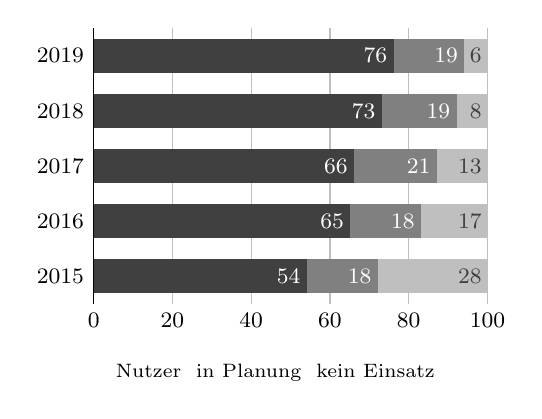
\begin{tikzpicture}[
			x=0.05cm, y=0.7cm
			]
			\foreach \x in {20,40,...,100}{
				\draw[color=lightgray] (\x, 0) node[below, color=black] {\footnotesize\x} -- (\x, 5);
			}
			
			\draw[color=lightgray, fill=lightgray] (0,4.2) rectangle +(100,0.6);
			\node[left, darkgray] at (101, 4.5) {\footnotesize 6};
			
			\draw[color=gray, fill=gray] (0,4.2) rectangle +(94,0.6);
			\node[left, white] at (95, 4.5) {\footnotesize 19};
			
			\draw[color=darkgray, fill=darkgray] (0,4.2) rectangle +(76,0.6);
			\node[left] at (0, 4.5) {\footnotesize 2019};
			\node[left, white] at (77, 4.5) {\footnotesize 76};
			
			
			\draw[color=lightgray, fill=lightgray] (0,3.2) rectangle +(100,0.6);
			\node[left, darkgray] at (101, 3.5) {\footnotesize 8};
			
			\draw[color=gray, fill=gray] (0,3.2) rectangle +(92,0.6);
			\node[left, white] at (93, 3.5) {\footnotesize 19};
			
			\draw[color=darkgray, fill=darkgray] (0,3.2) rectangle +(73,0.6);
			\node[left] at (0, 3.5) {\footnotesize 2018};
			\node[left, white] at (74, 3.5) {\footnotesize 73};
			
			
			\draw[color=lightgray, fill=lightgray] (0,2.2) rectangle +(100,0.6);
			\node[left, darkgray] at (101, 2.5) {\footnotesize 13};
			
			\draw[color=gray, fill=gray] (0,2.2) rectangle +(87,0.6);
			\node[left, white] at (88, 2.5) {\footnotesize 21};
			
			\draw[color=darkgray, fill=darkgray] (0,2.2) rectangle +(66,0.6);			
			\node[left] at (0, 2.5) {\footnotesize 2017};
			\node[left, white] at (67, 2.5) {\footnotesize 66};
			
			
			\draw[color=lightgray, fill=lightgray] (0,1.2) rectangle +(100,0.6);
			\node[left, darkgray] at (101, 1.5) {\footnotesize 17};
			
			\draw[color=gray, fill=gray] (0,1.2) rectangle +(83,0.6);
			\node[left, white] at (84, 1.5) {\footnotesize 18};
			
			\draw[color=darkgray, fill=darkgray] (0,1.2) rectangle +(65,0.6);
			\node[left] at (0, 1.5) {\footnotesize 2016};
			\node[left, white] at (66, 1.5) {\footnotesize 65};
			
			
			\draw[color=lightgray, fill=lightgray] (0,0.2) rectangle +(100,0.6);
			\node[left, darkgray] at (101, 0.5) {\footnotesize 28};
			
			\draw[color=gray, fill=gray] (0,0.2) rectangle +(72,0.6);
			\node[left, white] at (73, 0.5) {\footnotesize 18};
			
			\draw[color=darkgray, fill=darkgray] (0,0.2) rectangle +(54,0.6);
			\node[left] at (0, 0.5) {\footnotesize 2015};
			\node[left, white] at (55, 0.5) {\footnotesize 54};
			
			
			\draw (0, 0) node[below, color=black] {\footnotesize 0} -- (0, 5);
			
			\draw[draw=none] (0,0) -- (6,0) node[midway, xshift=6em, yshift=-2.5em] {\scriptsize \textcolor{darkgray}{$\blacksquare$} Nutzer \textcolor{gray}{$\blacksquare$} in Planung \textcolor{lightgray}{$\blacksquare$} kein Einsatz};
			
		\end{tikzpicture}
	}
	\caption{Einsatz von Cloud Computing in Unternehmen in Prozent \cite{heidkamp2020}}
	\label{tab:cloudanstieg}
\end{figure}


Das auch Unternehmen die Cloud Computing Technologie einsetzen dieser allerdings ebenfalls noch nicht völlig vertrauen, zeigt sich darin, dass in der Industrie viel Geld investiert wird, um die Sicherheit und den Schutz ihrer Cloud Ressourcen zu maximieren. So geht beispielsweise aus einer 2014 erschienen Umfragestatistik des Markforschungsunternehmens Vanson Bourne \cite{vansonbourne2014} hervor, dass 58\% aller befragten Unternehmen ihre jährlichen Ausgaben im Bereich der Cloud Sicherheit noch weiter erhöhen.

Welche Gefahren es konkret bei der Nutzung der Cloud gibt und welche Lösungsansätze es gibt um das Auftreten von Problemen zu minimieren sollen in dieser Ausarbeitung ergründet werden.

\section{Probleme des Cloud Computing}
Sicherheit und Schutz sind wichtige Eigenschaften die bei allen kommerziell genutzten Technologien beachtet werden müssen, um Probleme zu vermeiden. Dies gilt auch für alle Ressourcen des Cloud Computing. Gerade bei Anwendungen im öffentlichen Netz gibt es viele potenzielle Gefahren, die in der Industrie auch zu finanziellen Verlusten führen können. 
Dabei erstrecken sich die Gefahren von verlorenen Daten, über Betriebsspionage bis hin zu Hardwareschäden. 

\subsection{Fehlerhafter Schutz}
\label{sec:fehlender-Schutz}
Fehlender Schutz in Cloud Computing Diensten kann zu einem Problem für Cloud Nutzer aber auch für Cloud Anbieter werden. Im Folgenden wird auf grundsätzliche Gefahren eingegangen die durch fehlenden Schutz entstehen können.

Im Cloud Computing besteht die Gefahr von Accountdiebstählen oder gekaperte Services. 
Sobald Hacker sich Zugang zu einem Webservice der auf einem Cloud Server läuft, verschafft haben, 
können diese eigene Überwachungssoftware auf dem Service installieren 
und so bei gut genutzten Services in kurzer Zeit große Mengen sensibler Informationen von Nutzern des Service erhalten.
Da die Abhängigkeit von Cloud Computing jährlich zunimmt, 
steigt auch der Schaden solcher Hackerangriffe von Jahr zu Jahr \cite{jabbar2020}. 
 
Durch die hohe Dynamik die durch die Cloud geboten wird entstehen weitere neue Angriffsziele. So können zentral verwaltete Mikroservices, die für die Virtualisierung der Infrastruktur einzelner Nutzer eingesetzt werden zum Sicherheitsproblem werden, weil jeder Mikroservice eine andere Systemkonfiguration haben kann \cite{chen2019}. Somit kann jeder Mikroservice andere Sicherheitsrisiken bergen, die ausgenutzt werden können. Ist zudem keine logische Separierung der Ressourcen verschiedener Nutzer gegeben kann durch die Sicherheitslücke eines einzelnen Nutzers auch Schaden an der Cloud Infrastruktur anderer Nutzer verursacht werden \cite{wehrhahn-aklender2019}. In \autoref{fig:sicherheitsproblem} ist ein solcher Angriff dargestellt, bei dem sich durch die virtuelle Maschine eines Nutzers, aufgrund einer fehlenden Trennung der virtuellen Ressourcen, Zugang zu einem weiteren Nutzer verschafft werden konnte. 

\begin{figure}[b]
	\centering
	\includegraphics[width=\linewidth]{images/sicherheitsproblemneu.png}	
	\caption{Gefahr fehlender Trennung virtueller Ressourcen \cite{wehrhahn-aklender2019}}
	\label{fig:sicherheitsproblem}
\end{figure}

 Kann sich ein Angreifer Zugriff auf die Cloud Administration verschaffen hat dieser zudem möglicherweise Zugriff auf die Daten und Services aller Nutzer \cite{wehrhahn-aklender2019}.

Weitere Gefahren gehen von cross-site scripting, denial of service Angriffen, 
unsicher programmierten Anwendungen sowie 
data breaches, gehackte Interfaces und APIs, defekten Authentifizierungen 
und kompromittierten Berechtigungsnachweise aus. 
Letztere können insbesondere auch zu längeren Downtimes und einer reduzierten Verlässlichkeit führen, 
wodurch sich zukünftig die Gefahr von Downtimes erhöhen könnte \cite{jabbar2020}.

Gängige Sicherheitsprodukte eignen sich nur für Infrastrukturen deren Netzwerk-Konfigurationen sich nur selten ändern. Bei Cloud Computing können Sicherheitsgateways aufgrund der sich regelmäßig verändernden Infrastrukturen häufig  den Datenfluss des Netzwerks nicht ausreichend filtern \cite{wehrhahn-aklender2019}.

\subsection{Fehlende Zuverlässigkeit und Verfügbarkeit}
\label{sec:fehlende-Sicherheit}
Durch Ausfälle und um die Hochverfügbarkeit von Cloud Services gewährleisten zu können, 
kommt es jährlich zu Gewinneinbußen in dreistelliger Millionenhöhe \cite{snyder2015}.
Ausfälle von Cloud Services werden aufgrund eines besseren Netzausbaus, 
steigender Erfahrung und modernerer Softwarelösungen zwar seltener, 
können aber auch heute noch zu vereinzelten Ausfällen führen, die Imageschädigend wirken oder zu Einnahmeausfällen führen. 
So gab es zum Beispiel 2017 längere Ausfälle der Cloud Infrastruktur von 
IMB, GitLab, Facebook, Amazon Web Services, Microsoft Azure und Microsoft Office 365 \cite{tsidulko2017}.
Durch die Ausfälle kam es zu Datenverlusten sowie Zugriffsproblemen von Nutzern auf Accounts, 
Dienste, Projekte und auch kritischen Daten \cite{tsidulko2017}.
%Tsidulko J (2017) The 10 biggest cloud outages of 2017 (So far). 2017; https://www.crn.com/slide-shows/cloud/300089786/the-10-biggest-cloud-outages-of-2017-so-far.htm Accessed 1 Aug 2017

Trotz des fortschreitenden Netzausbaus, sowie besseren Technologien und damit einhergehend kürzeren Latenzzeiten kann es dennoch vorkommen, dass es zu höheren Latenzen durch einen schlechten lokalen Netzausbau, Störungen oder Überlastungen kommen kann.
Während es bei lokalen Anwendungen keine Latenzen gibt, können Latenzen zwischen Nutzer und Cloudinfrastruktur die Benutzerfreundlichkeit von Anwendungen reduzieren, wodurch diese weniger attraktiv gegenüber lokalen Anwendungen wirken können.
Ebenfalls ist es unter Umständen möglich, dass gesendete oder empfangene Datenpakete verloren gehen oder kompromittiert werden und so die Zuverlässigkeit reduziert wird. 

Latenzen können auch innerhalb der Cloud auftreten, weil nicht unbedingt garantiert wird, dass die für die Cloud Infrastruktur benötigten Ressourcen auf derselben Hardware bereitgestellt wird. 
Die physikalische Entfernung und die Anzahl an Switches die beim Datenaustausch mit den verteilten Ressourcen auch innerhalb der Cloud Infrastruktur durchquert werden muss, kann je nach Anwendungsfall die Ausführungszeit erhöhen.
Auf diese Art können Anwendungen, von denen eine schnelle Ausführungszeit als Teil ihrer Zuverlässigkeit erwartet wird, ausgebremst werden. Davon sind insbesondere Dienste betroffen die sich mit anderen Diensten austauschen. Eine solche Interaktion ist in \autoref{fig:infrastruktur} dargestellt. Die rot markierten Interaktionen zeigen die zusätzlich durch Latenzen belasteten Verbindungen. 

\begin{figure}[b]
	\centering
	\includegraphics[width=\linewidth]{images/cloudstruktur.png}	
	\caption{Interaktionsszenario innerhalb einer Cloud-Infrastrukur}
	\label{fig:infrastruktur}
\end{figure}

Auch von außen kann die Verfügbarkeit der Cloud Services negativ beeinträchtigt werden. So kann durch einen DDoS Angriff versucht werden einem Service zu schaden. Dabei treten zwei Arten von Angriffen auf. In den meisten Fällen wird dabei von außerhalb der Cloud versucht die Verfügbarkeit von Clouddiensten durch Überlastung negativ zu beeinflussen \cite{darwish2013}. Seltener wird versucht von innerhalb der Cloud physikalische Ressourcen wie Netzwerke, Bandbreite, Speicherplatz oder Datenbanken anzugreifen \cite{darwish2013}.

\subsection{Datenschutz}
Auch der Wunsch der Benutzer nach Datenschutz ist eine Herausforderung im Cloud Computing. Die Nutzung von Cloud Computing birgt generell datenschutzrechtliche Risiken \cite{selzer2020}. 
Persönliche Daten von Nutzern der Clouddienste werden von deren Anbietern gehandhabt und nicht lokal gespeichert. 
Diese Anbieter sind oft internationale Unternehmen, mit Servern die über mehrere Länder verteilt sein können. Je nach Land, in dem die Server stehen, gelten eventuell auch andere Richtlinien wie die Sicherheit der Daten gewährleistet werden müssen \cite{selzer2020}.

Daten der Cloud unterliegen generell dem Risiko, dass andere Nutzer diese einsehen könnten \cite{ali2015}. 
Die Herausforderungen des Cloud Computing an die Kommunikation über das Internet unterscheiden sich jedoch nicht von der konventionellen Kommunikationen über das Internet \cite{ali2015}. 
Allerdings gibt es in der Cloud auch Kommunikationen innerhalb der Cloud Infrastruktur. Diese neue Art der Kommunikation wird von den Anbietern selbst überwacht und ist entsprechend für den Nutzer der Cloud nicht transparent in Bezug auf die Übertragungssicherheit \cite{ali2015}. 
So können Administratoren der Cloud durch den Einsatz unzureichender Konfigurationswerkzeuge eventuell nicht den geforderten Sicherheitsstandard für die Übertragung erreichen ohne dass der Nutzer dies erfährt \cite{dinh2013}.
Durch die geteilten Ressourcen der Cloud Infrastruktur kann es ebenfalls zu Datenschutzrisiken kommen, weil diese Ressourcen gegebenenfalls nicht ausreichend bereinigt sind und Informationen des vorherigen Nutzers der Ressourcen für den neuen Nutzer zugängig sind. So konnte von Balduzzi et al. \cite{balduzzi2012} durch die Nutzung von Datenwiederherstellungstechniken auf die Amazon Elastic Compute Cloud in 98\% aller Fälle Daten des vorherigen Nutzers wiederhergestellt werden. 

\section{Lösungsansätze}
Wie aus dem vorhergehenden Kapitel hervorgeht, gibt es im Cloud Computing einige Probleme, die es zu behandeln gilt, um die Gefahren für Cloudanbieter und deren Nutzer zu neutralisieren oder zumindest zu reduzieren. 
Für eine Vielzahl der genannten Probleme gibt es Lösungsansätze die in der Praxis auch bereits eingesetzt werden. 
Viele der genannten Probleme lassen sich durch ein fehlertoleranteres System und eine erhöhte Datensicherheit behandeln. Im Folgenden werden deshalb Ansätze aufgezeigt, um diese beiden Ziele zu erreichen.

\subsection{Fehlertolerante Systeme}
Um Datenverluste zu vermeiden und die Verfügbarkeit zu maximieren ist es notwendig, fehlertolerantere Systeme aufzubauen. Dazu wurden von Mesbahi \cite{mesbahi2018} aus den Arbeiten von Ganesh et al. \cite{ganesh2014} sowie Jhawar et al. \cite{jhawar2013} die folgenden Maßnahmen zusammengetragen.

\begin{itemize}
\item
Präventives Migrieren: Beinhaltet das Speichern der Zustände eines Prozesses, das Abschalten von Prozessen, die Überführung dieses Zustands zu einem anderen Knoten und die dortige Wiederaufnahme des abgeschalteten Prozesses.
Dabei wird ein System eingesetzt, das den Zustand des Prozesses durch Feedbacks regelmäßig überwacht und analysiert. 
\item
Software Verjüngung: Eine Vorbeugende Maßnahme damit sich keine Altlasten in der laufenden Software ansammeln können. Dabei wird die eingesetzte Software periodisch neu gestartet, um zu vermeiden, dass die Software durch verbliebene Altlasten nach und nach Fehler entstehen.
\item
Checkpointing: Durch regelmäßiges Zwischenspeichern des aktuellen Zustands einer Anwendung soll im Falle eines Fehlers die Anwendung wieder in den Zustand zu einem Zeitpunkt gebracht werden können, zu dem die Anwendung fehlerfrei lief. Dadurch wird vermieden, dass die Anwendung in einem Fehlerfall noch einmal komplett von Anfang an gestartet werden muss. In einem Fehlerfall wird somit weniger Fortschritt verloren und rechenintensive Schritte müssen eventuell nicht erneut ausgeführt werden.
\item
Redundanz: Durch Vervielfachung von Services und Daten kann eine bessere Ausfallsicherheit gewährleistet werden, weil im Falle eines Fehlers auf einer fehlerfreien Kopie des Service weitergearbeitet werden kann. Die Kopien können zudem auf unterschiedliche Systeme aufgeteilt werden, wodurch bei einem Ausfall eines Systems der Service in Form einer identischen Kopie weiterhin zur Verfügung steht.
\item
Erneutes Übertragen: Durch erneutes Übertragen eines fehlgeschlagenen Auftrags an denselben oder einen anderen Host erhält der Service eine weitere Chance den Auftrag korrekt zu verarbeiten. Im Falle eines Netzwerkproblems bei der Übertragung des Auftrags kann so noch einmal derselbe Auftrag versendet werden, in der Hoffnung, dass es dieses Mal zu keinem Netzwerkproblem kommen wird und der Auftrag korrekt ausgeführt wird. Ein Benutzer erfährt durch eine schnelle Ausführung eines erneuten Sendens eventuell gar nicht, dass der ursprüngliche Auftrag fehlgeschlagen ist.
\end{itemize}

Durch fehlertolerantere Systeme lässt sich also die Chance reduzieren, dass Teile der Cloud in einen fehlerhaften Zustand geraten oder, wenn sie dennoch in einen Fehlerzustand geraten sind, dieser möglichst geringe Auswirkungen auf das System hat und einfach oder sogar automatisiert behoben werden kann.

\subsection{Datensicherheit} 
Um kritische oder private Daten besser zu schützen gibt es einige Ansätze. Im Folgenden wurden einige dieser Ansätze zusammengetragen und erklärt. Generell gilt, je mehr der Ansätze im Cloud Computing berücksichtigt werden, desto besser können kritische oder private Daten bewahrt werden.
\begin{itemize}
\item
Verschlüsseln von physischen Festplatten: Durch das Verschlüsseln von physischen Datenträgern lassen sich die Folgen eines widerrechtlichen Datenabrufs reduzieren, im Falle eines Datenraubs können die geraubten Informationen eventuell gar nicht oder nur mit beträchtlichem Aufwand missbraucht werden \cite{selzer2020}.
\item
Verschlüsseln der Datenübertragung: Durch die Verschlüsselung der Datenübertragung zwischen Cloud Anwendung und Nutzer lässt sich die Gefahr eines Datendiebstahls über eine unsichere Verbindung reduzieren. So können bereits bei der Verschlüsselung physikalischer Datenträger erbeutete Daten nur mit beträchtlichem Aufwand missbraucht werden \cite{selzer2020}.
\item
Pseudonymisierung: Durch die Verschlüsselung von persönlichen Nutzerdaten kann deren  Personenbezug entfernt werden, um einen höheren Grad der Anonymisierung bei der Verarbeitung und Speicherung zu erreichen \cite{selzer2020}.
\item
Kontrollen über Zertifikate oder vor Ort: Durch die vermehrte Kontrolle von Zertifikaten von Dritten oder vor Ort bei Anbietern, lässt sich die Korrektheit der Datenverarbeitung bedingt sicherstellen. Nutzer können sich selbst vergewissern, ob ihr Service datensicherheitskonform arbeitet und dass die sich auf den Servern befindlichen Daten ausreichend gegen äußere Einflüsse geschützt sind \cite{selzer2020}. 
\item 
Datenmetriken: Der Grad des Datenschutzes lässt sich durch Datenmetriken aus Logdaten automatisiert ermitteln. Der Einsatz solcher Metriken erfordert dabei weniger Fachwissen des Prüfers als es bei einer vor Ort Kontrolle benötigt würde, weil das Fachwissen durch die Metriken geliefert wird \cite{selzer2020}. Eine Erweiterung der durch die Metriken erfassten Daten kann dabei zusätzlich mit individuellen Anforderungen ergänzt werden \cite{selzer2020}. Die Datenmetriken lassen sich dabei regelmäßig ausführen, wodurch der Nutzer aktuelle und zeitnahe Informationen über den Zustand der Datensicherheit seines Systems erhält und gegebenenfalls ebenso zeitnah auf Verstöße reagieren kann \cite{selzer2020}.
\item 
Regelmäßige Backups: Durch das regelmäßige Abspeichern des gesamten Datenbestands lässt sich das Risiko von Datenverlusten reduzieren, indem im Falle eines Hardwareausfalls mithilfe der Backupdaten ein Großteil des Datenbestandes wiederhergestellt werden kann \cite{wehrhahn-aklender2019}.
\item
Regelmäßige Updates: Durch automatisierte Updates können Cloudservices aktuell gehalten werden. Durch häufige automatisierte Updates wird die Zeit zwischen den einzelnen Updates reduziert, wodurch die Sicherheit des Service auf dem neusten Stand ist und weniger Sicherheitslücken ausgenutzt werden können \cite{wehrhahn-aklender2019}.
\item
Standardisierte Angebote: Durch standardisierte Cloud Computing Angebote kann eine höhere Nachvollziehbarkeit im Fehlerfall erreicht werden. Außerdem können Anomalien bei einzelnen Nutzern schneller festgestellt und behandelt werden \cite{wehrhahn-aklender2019}.
\end{itemize}

Somit zeigt sich, dass es bereits umfangreiche Maßnahmen zur Bewahrung kritische oder private Daten im Cloud Computing gibt, jedoch keiner der Ansätze allein die Daten der Cloud ausreichend sichern kann.


\section{Fazit}
Die von vor Ort Kontrollen durchgeführte Sicherstellung der Datenschutzkonformität hat in ihrer Anwendung nicht die erwünschten Ergebnisse gebracht, weil sich Anbieter auf Kontrollen vorbereiten und Mängel im Vorfeld aus dem Weg geräumt haben \cite{selzer2020}.
Die Qualität von Zertifikaten von Drittanbietern lässt sich nicht immer mit Sicherheit bestimmen, weil es je nach Land sehr viele unterschiedliche Datenschutz und Datensicherheitszertifizierungen geben kann \cite{selzer2020}.

Durch ein standardisiertes Angebot lassen sich viele Sicherheitsrisiken des Cloud Computing reduzieren. So ermöglicht eine Standardisierung regelmäßigere Updates für alle Nutzer, weil sich Anbieter auf die Perfektion ihres Angebotes spezialisieren können. Das erleichtert es sowohl den Nutzern als auch dem Anbieter die Vorgänge in der Cloud nachzuvollziehen und Sicherheitslücken zu erkennen. 

Die vielseitigen Angriffsmöglichkeiten auf die Cloud lassen sich, selbst nach Anpassungen an die Cloudstruktur nicht mit einem einzelnen IT-Sicherheitsprodukt absichern, ohne dass dadurch die Funktion eingeschränkt wird. So können Sicherheitsgateways nur dann den Datenfluss der Cloud ausreichend filtern, wenn sich die Infrastruktur der Cloud nicht weiter verändert. Das würde bedeuten, dass keine dynamische Migration von Ressourcen der Cloud erfolgen dürfte wodurch Skalierbarkeit sowie Verfügbarkeit stark eingeschränkt werden würde \cite{wehrhahn-aklender2019}.

Zusammenfassen lässt sich sagen, dass über die vergangenen Jahre viele Probleme des Cloud Computings aufgedeckt wurden. Der größte Teil davon lässt sich durch bereits existierende Lösungsansätze vermeiden oder stark reduzieren. Dass es dennoch Firmen gibt, die Cloud Computing noch nicht einsetzen lässt sich darauf zurückführen, dass es zwar Lösungen für die gefundenen Probleme gibt, diese allerdings größtenteils von den Cloud Anbietern umgesetzt werden müssen. Gerade kleine Firmen oder privaten Nutzern fehlt oft das Wissen und der Einfluss sicherzustellen, ob die von Anbietern bereitgestellten Cloudstrukturen alle erforderlichen Maßnahmen getroffen haben um die Daten des Nutzers sowie der Zuverlässigkeit und Verfügbarkeit seiner Clouddienste zu gewährleisten.

\subsection{Ausblick}
Da in den vergangenen Jahren das Thema Datenschutz auch für Privatpersonen immer mehr an Bedeutung gewonnen hat ist anzunehmen, dass aufgrund dessen auch die Cloud Anbieter diesem Bedürfnis nachkommen werden und verstärkt auf die Datensicherheit ihrer Angebote achten werden. 
Da auch die Konkurrenz unter Cloud Anbietern zunimmt, ist es wahrscheinlich, dass diese die Qualität ihrer Angebote weiter erhöhen werden, um weiterhin konkurrenzfähig zu bleiben.
Sicherheitslücken und Ausfälle werden in der Öffentlichkeit zunehmend auf Cloud Anbieter zurückgeführt werden. Dadurch wird auch der Druck auf die Cloud Anbieter steigen, eine hohe Qualität ihrer Angebote zu garantieren.
Es ist daher anzunehmen, dass der Einsatz von Cloud Computing in der Industrie auch weiterhin steigen wird, weil die Qualität der Cloud weiter zunimmt, und die Bedenken der Industrie immer weniger Gewicht haben werden.

